\documentclass{classrep}
\usepackage[utf8]{inputenc}


\studycycle{Informatyka, studia dzienne, inż I st.}
\coursesemester{V}
\coursename{Obliczenia naukowe}
\courseyear{2017/2018}
\courseteacher{dr hab. Paweł Zieliński}
\coursegroup{czwartek TN, 11:15}

\author{
  \studentinfo{Agata Jasionowska}{229726}
}

\title{Laboratorium \ppauza Lista 5}

\DeclareMathOperator{\sgn}{sgn}
\newcommand{\mA}{\bm{A}}
\newcommand{\mB}{\bm{B}}
\newcommand{\mC}{\bm{C}}
\newcommand{\mL}{\bm{L}}
\newcommand{\mU}{\bm{U}}
\newcommand{\mZ}{\bm{0}}
\newcommand{\vb}{\bm{b}}
\newcommand{\vx}{\bm{x}}
\newcommand{\vz}{\bm{z}}
\newcommand{\vp}{\bm{p}}
\newcommand{\R}{\mathbb{R}}

\begin{document}

\maketitle

\section{Zadanie 1}	
	\subsection{Opis problemu}
		Zadanie dotyczyło rozwiązania układu równań liniowych:
		$$\mA\vx = \vb,$$
		dla danej macierzy współczynników $\mA \in \R^{n\times n}$ i wektora prawych stron $\vb \in \R^n$, $n \geq 4$ metodą eliminacji Gaussa 	(bez wyboru elementu głównego oraz z częściowym wyborem elementu głównego) oraz obliczeniu rozkładu $\mL \mU$ macierzy i rozwiązaniu z jego wykorzystaniem układu $\mA \vx = \vb$.
		
		Macierz $\mA$ jest rzadka i blokowa o następującej strukturze:
		$$
			\mA =
			\left(\begin{array}{ccccccc}
			\mA_1 & \mC_1 & \mZ & \mZ & \mZ & \cdots & \mZ \\
			\mB_2 & \mA_2 & \mC_2 & \mZ & \mZ  & \cdots & \mZ \\
			\mZ  & \mB_3 & \mA_3 & \mC_3 & \mZ  & \cdots & \mZ \\
			\vdots & \ddots & \ddots & \ddots & \ddots & \ddots & \vdots\\
			\mZ   & \cdots & \mZ  & \mB_{v-2} & \mA_{v-2} & \mC_{v-2} & \mZ \\
			\mZ  & \cdots & \mZ  &  \mZ &\mB_{v-1} & \mA_{v-1} & \mC_{v-1}  \\
			\mZ  & \cdots & \mZ & \mZ & \mZ& \mB_{v} & \mA_{v}  \\
			\end{array}\right),
		$$
		gdzie $v = \frac{n}{\ell}$, $l | n$, a $\ell \geq 2$ jest rozmiarem wszystkich bloków $\mA_k$, $\mB_k$, $\mC_k$ macierzy $\mA$. 
		
		Struktura wewnętrznych bloków $\mA_k$, $\mB_k$, $\mC_k$ macierzy $\mA$ jest następująca:
		\begin{enumerate}[(a)]
			\item $\mA_k \in \R^{\ell\times \ell}$,   $k = 1, \ldots,v$ są macierzami gęstymi,
			\item $\mB_k \in \R^{\ell\times \ell}$,   $k = 2, \ldots,v$ są postaci:
			$$
				\mB_k =
				\left(\begin{array}{ccccc}
				0 & \cdots & 0 & b_{1\,\ell-1}^k & b_{1\,\ell}^k \\
				0 & \cdots & 0 & b_{2\,\ell-1}^k & b_{2\,\ell}^k \\
				\vdots & & \vdots & \vdots & \vdots \\
				0 & \cdots & 0 & b_{\ell\,\ell-1}^k & b_{\ell\,\ell}^k \\
				\end{array}\right),
			$$ 
			\item $\mC_k \in \R^{\ell\times \ell}$,   $k = 1, \ldots,v\!-\!1$ są diagonalne:
			$$
				\mC_k =
				\left(\begin{array}{ccccc}
				 c_{1}^k & 0 & 0 & \cdots & 0  \\
				0 &  c_{2}^k &  0 & \cdots & 0  \\
				\vdots &  \ddots &  \ddots & \ddots & \vdots  \\
				0 & \cdots & 0 &  c_{\ell-1}^k & 0 \\
				0 & \cdots & 0 &  0 & c_{\ell}^k \\
				\end{array}\right),
			$$ 
		\end{enumerate}
\section{Sposób rozwiązania}
	\subsection{Wykorzystanie pamięci}
		% v * l *l + (v-1) * l * 2 + (v-1)*l = n *l + v * l * 2 - l * 2 + v * l - l = nl + 2n - 2l + n - l = ln + 3n - 3l = ln + 3(n-l)

	W konstruowaniu rozwiązania problemu niezwykle istotny był odpowiedni sposób przechowywania macierzy w pamięci.
	
	Zważywszy na to, iż $\mA$ jest macierzą rzadką (tylko $n \ell + 3(n - \ell)$ elementów niezerowych --- $\ell^2$ w każdym z $v$ bloków $\mA_k$, $2\ell$ w każdym z $v-1$ bloków $\mB_k$ i $\ell$ w każdym z $v-1$ bloków $\mC_k$), to istnieje sposób na zapamiętanie jej znacznie efektywniej, niżby to miało miejsce w przypadku dwuwymiarowej tablicy $n\times n$. 
	
	W implementacji skorzystano z dostępnej w języku \texttt{Julia} struktury \texttt{SparseMatrixCSC}, gdzie macierze przechowywane są w skompresowanym porządku kolumnowym. Pozwala to na jeszcze jedną optymalizację, bazującą na fakcie, że czas dostępu do elementów jest krótszy, jeśli poruszamy się wzdłuż kolumn. Skoro opisywany algorytm eliminacji Gaussa ma przebieg wierszowy, więc przechowywane w pamięci macierze są zawsze transponowane. W dalszych rozważaniach jednak, dla ułatwienia, macierze indeksowane są w sposób standardowy, gdyż różnica polega wyłącznie na zamianie miejscami indeksów wiersza i kolumny.
	
	\subsection{Eliminacja Gaussa}
		\subsubsection{Podstawy teoretyczne}
		Metoda eliminacji Gaussa to algorytm rozwiązywania układów równań liniowych, obliczania rzędu macierzy i wartości wyznacznika oraz wyznaczania rozkładu LU, wykorzystując operacje elementarne. 
		
		W sposobie rozwiązywania układu równań tą metodą wyróżnić można dwa główne etapy. Pierwszym z nich jest sprowadzenie układu do układu równoważnego z macierzą trójkątną górną. Algorytm będzie polegał na zerowaniu kolejnych elementów znajdujących się pod diagonalą. Przykładowo w celu wyzerowania elementu $a_{i1}$ od $i$-tego wiersza zostanie odjęty pierwszy wiersz  pomnożony przez $z=a_{i1}/a_{11}$ (liczba ta nazywana dalej będzie \emph{mnożnikiem}). W ten sposób w pierwszym kroku wyzerowane zostają wszystkie elementu poniżej pierwszego wiersza w pierwszej kolumnie, dalej powtarzane jest to dla drugiej kolumny, itd. Warto zwrócić uwagę na fakt, iż procedura zawiedzie w sytuacji, gdy na diagonali pojawi się zero. Algorytm wymaga wtedy do poprawnego działania pewnej modyfikacji, np. zamiany miejscami wierszy.
		
		Drugim i ostatnim etapem rozwiązywania układu równań jest zastosowanie algorytmu zwanego $algorytmem~podstawiania~wstecz$. Opiera się on w głównej mierze na zastosowaniu wzoru
			$$n_i = \frac{b_i-\sum_{j=i+1}^n{a_{ij}}}{a_{ii}}$$
		do kolejnych $i$-tych wierszy macierzy, rozpoczynając od ostatniego z nich.
		
		W tym miejscu warto także wspomnieć o złożoności obliczeniowej. Otóż algorytm eliminacji Gaussa cechuje złożoność rzędu $O(n^3)$, zaś podstawianie wstecz z kroku drugiego --- $O(n^2)$. Prowadzi to do konkluzji, że w celu rozwiązania układu równań należy wykonać $O(n^3)$ operacji.
		
		\subsubsection{Rozwiązywanie układów równań}
			W sposobie rozwiązania uwzględniona została charakterystyczna, trójdiagonalno blokowa postać macierzy $\mA$, co pozwoliło na znaczne zredukowanie liczby potrzebnych do wykonania operacji w stosunku do rozwiązania z zastosowaniem standardowego algorytmu eliminacji Gaussa. Otóż należy zauważyć, że nie jest konieczne wyzerowanie wszystkich elementów znajdujących się w danej kolumnie pod diagonalą. Dla pierwszych $\ell-2$ kolumn niezerowe elementy mogą się znajdować jedynie w pierwszych $\ell$~rzędach (są to tylko elementy bloku~$\mA_1$), dla kolejnych $\ell$ kolumn  niezerowe elementy mogą się znajdować w pierwszych $2\ell$~rzędach (dwie ostatnie kolumny bloku~$\mB_2$ oraz elementy bloku~$\mA_3$), w kolejnych $\ell$ kolumnach niezerowe elementy będą się znajdowały w pierwszych $3\ell$~rzędach (niezerowe elementy bloku~$\mB_3$ oraz elementy bloku $\mA_4$)~itd.
			
	W ostatnich $\ell$ rzędach to $\mA_v$ jest leżącym najbardziej z prawej blokiem, a więc ostatnie niezerowe elementy leżą w kolumnie $n$-tej.
	Pozwala to na zbudowanie wzoru na maksymalny indeks kolumny, w której w danym rzędzie znajduje się niezerowy element:
	$$
	last_c(row) = \min\{n,~row + \ell\}.
	$$
	
	Ponadto, jeśli w którymś z etapów metody eliminacji Gaussa następuje odjęcie podanego rzędu od znajdujących się poniżej to nie następuje modyfikacja elementów w kolumnach o indeksach większych niż $last_c(row)$.
	
	Bazując na spostrzeżeniach przedstawionych powyżej, indeks ostatniego niezerowego elementu danej kolumny można wyliczyć jako:
	$$
	last_r(column) = \min\left\lbrace n,~\ell + \ell \cdot \left \lfloor\frac{column + 1}{\ell}\right \rfloor\right\rbrace
	$$
	
	Warte zauważenia jest także to, iż w każdym wierszu (poza $\ell$ ostatnimi elementami) ostatni niezerowy element należy do diagonali bloku $\mC_i$. Elementy te są zawsze odległe o $\ell$ od elementów diagonalnych całej macierzy. Finalnie eliminacja Gaussa doprowadziła do otrzymania układu z macierzą trójkątną górną, na którego rozwiązanie pozwala już algorytm podstawiania wstecz.
	
	Złożoność obliczeniowa całej metody, przyjmując $\ell$ jako stałą, wynosi $O(n)$ (liczba przebiegów wszystkich pętli to: $(n-1) \cdot 2\ell \cdot \ell + n \cdot l$).
	
	Szczegółowy przebieg opisywanej metody przedstawia Algorytm \ref{alg:gauss}.
	
	
	\begin{algorithm}[h]
	    			\SetKwInOut{Input}{Input}
	    			\SetKwInOut{Output}{Output}
	    			\SetKwProg{Fn}{Function}{}{}
	    			\SetKw{KwDownTo}{downto}
	    			\SetKw{Err}{error}
	    			
				\SetKwData{L}{$\ell$} 			
				\SetKwData{N}{$n$}    				
				\SetKwData{B}{$\vb$}    		
				\SetKwData{A}{$\mA$}    			
	    			\SetKwData{X}{$\vx$}
	    			\SetKwData{F}{f}
	    			\SetKwData{Z}{z}
	    			\SetKwData{I}{i}
	    			\SetKwData{J}{j}
	    			\SetKwData{K}{k}
	    			\SetKwData{Sum}{sum}
	    			\SetKwData{Col}{$lastC$}
	    			\SetKwData{Row}{$lastR$}
				\SetKwFunction{ge}{gauss}
				\SetKwFunction{Min}{$\min$}
	
				\footnotesize
			    \Input{\\
			    \begin{tabular}{rcl}
		  			{\A} & ---& macierz,\\
		  				{\B} & --- & wektor prawych stron, \\
		  			{\N} &---& rozmiar macierzy \A, \\
		  			{\L} & --- & rozmiar bloku macierzy \A.  		
				\end{tabular}
				}
			    \Output{\\
			    \begin{tabular}{rcl}
		    			{\X}& ---& wektor długości \N zawierający pierwiastki układu $\A\X=\B$.
				\end{tabular}		    			
			    	}
			    	\Fn{\ge{\A,~\B,~\N,~\L}}{
			    		\For{$\K \gets 1$ \KwTo $\N-1$} {
			    		$\Col\gets \Min(\K + \L, \N)$\;
			    		$\Row\gets\Min\left(\L + \L \cdot \left \lfloor\frac{\K + 1}{\ell}\right \rfloor, n\right)$\;
			    		\For{$\I \gets \K+1$ \KwTo \Row}{
			    			\If{$\A[\K][\K] = 0$}{\Err Diagonal coefficient is equal zero.}
			    			$\Z \gets \A[\I][\K] / \A[\K][\K]$\;
			    			$\A[\I][\K] \gets 0 $ \;
			    			\For{$\J \gets \K+1$ \KwTo \Col}{
			    				$\A[\I][\J] \gets \A[\I][\J] - \Z \cdot \A[\K][\J]$\;
			    			}
			    			$\B[\I] \gets \B[\I] - \Z \cdot \B[\K]$\;
			    		}
			    		}
			   \For{$\I \gets \N$ \KwDownTo $1$}{
			   		$\Sum \gets 0$\;
			   		$\Col\gets \Min(\I+ \L, \N)$\;
			   		\For{$\J \gets \K+1$ \KwTo $\Col$}{
					$\Sum \gets \Sum + \X[\I] \cdot \A[\I][\J]$\;
			   		}
			   		$\X[\I] \gets (\B[\I] - \Sum) / \A[\I][\I]$\;
			   }
			   		   
	    			\KwRet \X\;
				}
	\caption{Metoda eliminacji Gaussa.}\label{alg:gauss}
	\normalsize
	\end{algorithm} 
	
	\subsubsection{Wariant z wyborem elementu głównego}
		Powyżej została przedstawiona metoda eliminacji Gaussa bez wyboru elementu głównego. W pewnych sytuacjach przydatny bywa także jej wariant z częściowym wyborem, umożliwiając rozwiązywanie układów z zerami na diagonali. W praktyce stosuje się następująco: wybrany zostaje wiersz, dla którego element z eliminowanej obecnie kolumny $k$ ma największą wartość (co do modułu), a następnie zamieniony z $k$-tym wierszem; dalsze kroki pozostają bez zmian.
		
		Takie działanie może być bardzo kosztowne dla macierzy o dużych rozmiarach, stąd właśnie informacja, na której pozycji w macierzy znajduje się obecnie dany wiersz przechowywana jest w dodatkowym wektorze ($p$). Zmiana w samym algorytmie jest niewielka - odwołanie do konkretnego wiersza zastąpione zostało odwołaniem do odpowiadającej pozycji w wektorze permutacji.
		
		Kolejnym z problemów jest prawidłowe określenie granicznego $last_c$. Zaobserwować można, że podczas eliminowania współczynników z $\ell - 2$ pierwszych kolumn najdalszy niezerowy element można stworzyć w kolumnie z indeksem $2\ell$ --- poprzez odejmowanie $\ell$-tego wiersza, który w tej kolumnie posiada niezerowy element. Podczas eliminowania współczynników z kolejnych $\ell$ kolumn najdalszy niezerowy element można stworzyć w kolumnie z indeksem $3\ell$, analogicznie poprzez odejmowanie $2\ell$-tego wiersza, który w tej kolumnie posiada niezerowy element. Zgodnie z tym rozumowaniem nowy wzór będzie miał następującą postać:
			$$
			last_c(row) = \min\ \left\lbrace n,~2\ell + l \cdot \left \lfloor\frac{row + 1}{\ell} \right \rfloor \right\rbrace.
			$$

		Identycznie  ograniczenie zostało nałożone dla wykonywania algorytmu podstawiania wstecz. Brak nowych niezerowych elementów poza tymi już uwzględnionymi, a jedyną zmianą jest więcie pod uwagę permutacji wiersza.
		
		Złożoność obliczeniowa wariantu z częściowym wyborem elementu głównego jest gorsza niż poprzednio przedstawiona standardowa eliminacja Gaussa (ograniczenia nałożone na $last_c$). Ostatecznie jednak, przy założeniu, że $\ell$ jest stałe, nie wpływa to na osiągnięcie złożoności większej niż $O(n)$.
		
		Szczegóły implementacji metody eliminacji Gaussa z wyborem elementu głównego przedstawia Algorytm \ref{alg:pivotgauss}.


	\begin{algorithm}[h]
				\LinesNumbered
	    			\SetKwInOut{Input}{Input}
	    			\SetKwInOut{Output}{Output}
	    			\SetKwProg{Fn}{Function}{}{}
	    			\SetKw{KwDownTo}{downto}
	    			\SetKw{Err}{error}
	    			
				\SetKwData{L}{$\ell$} 			
				\SetKwData{N}{$n$}    				
				\SetKwData{B}{$\vb$}    		
				\SetKwData{A}{$\mA$}    			
	    			\SetKwData{X}{$\vx$}
	    			\SetKwData{F}{f}
	    			\SetKwData{Z}{z}
	    			\SetKwData{I}{i}
	    			\SetKwData{J}{j}
	    			\SetKwData{K}{k}
	    			\SetKwData{Mm}{m}
	   			\SetKwData{P}{p}
	   			\SetKwData{Q}{q}
	    			\SetKwData{Sum}{sum}
	    			\SetKwData{Idx}{idx$_{\max}$}
	    			\SetKwData{Val}{val$_{\max}$}
	    			\SetKwData{Col}{$lastC$}
	    			\SetKwData{Row}{$lastR$}
				\SetKwFunction{ge}{gauss\_with\_pivot}
				\SetKwFunction{Min}{$\min$}
				\SetKwFunction{Swap}{swap}
	
				\footnotesize
			    \Input{\\
		    \begin{tabular}{rcl}
	  			{\A} & ---& macierz,\\
	  				{\B} & --- & wektor prawych stron, \\
	  			{\N} &---& rozmiar macierzy \A, \\
	  			{\L} & --- & rozmiar bloku macierzy \A.  		
			\end{tabular}
				}
			    \Output{\\
			    \begin{tabular}{rcl}
	    			{\X}& ---& wektor długości \N zawierający pierwiastki układu $\A\X=\B$.
				\end{tabular}		    			
			    	}
			    	\Fn{\ge{\A,~\B,~\N,~\L}}{
			    		$\P \gets \{\I : \I \in \{1, \ldots, n \} \}$\;
			    		\For{$\K \gets 1$ \KwTo $\N-1$} {
			    		$\Row\gets\Min\left(\L + \L \cdot \left \lfloor\frac{\K + 1}{\ell}\right \rfloor\!, n\right)$\;
			    		$\Col\gets \Min\left(2\L + \L \cdot \left \lfloor\frac{\K + 1}{\ell}\right \rfloor\!, \N\right)$\;
			    		\For{$\I \gets \K+1$ \KwTo \Row}{
			    			$\Idx \gets \Mm$ takie, że: $\A[\P[\Mm]][\K] = \max(|\A[\P[\Q]][\K]| : \Q \in \{\I, \ldots,\Row\} )$\;
			 		
			    			\If{$\P[\Idx] = 0$}{\Err Singular matrix.}
			    			\Swap($\P[\K], \P[\Idx]$)\;
			    			$\Z \gets \A[\P[\I]][\K] / \A[\P[\K]][\K]$\;
			    			$\A[\P[\I]][\K] \gets 0 $ \;
			    			\For{$\J \gets \K+1$ \KwTo \Col}{
			    				$\A[\P[\I]][\J] \gets \A[\P[\I]][\J] - \Z \cdot \A[\P[\K]][\J]$\;
			    			}
			    			$\B[\P[\I]] \gets \B[\P[\I]] - \Z \cdot \B[\P[\K]]$\;
			    		}
			    		}
			   \For{$\I \gets \N$ \KwDownTo $1$}{
			   $\Sum \gets 0$\;
			   		$\Col\gets \Min\left(2\L + \L \cdot \left \lfloor\frac{\I + 1}{\ell}\right \rfloor\!, \N\right)$\;
			   		\For{$\J \gets \K+1$ \KwTo $\Col$}{
					$\Sum \gets \Sum + \X[\J] \cdot \A[\P[\I]][\J]$\;
			   		}
			   		$\X[\I] \gets (\B[\P[\I]] - \Sum) / \A[\P[\I]][\I]$\;
			   }
			   		   
	    			\KwRet \X\;
				}
	\caption{Metoda eliminacji Gaussa z częściowym wyborem elementu głównego.}\label{alg:pivotgauss}
	\normalsize
	\end{algorithm} 	
	
	\subsection{Rozkład LU}
		\subsubsection{Podstawy teoretyczne}
		Rozkład $\mL \mU$ macierzy $\mA$ to przedstawienie zadanej macierzy w postaci iloczynu $\mA = \mL \mU$, gdzie $\mL$ jest macierzą trójkątną dolną, zaś $\mU$ --- macierzą trójkątną górną. Dodatkowym założeniem jest, że wszystkie diagonalne elementy $\mL$ to 1. 
		
		Na uzyskanie rozkładu $\mL \mU$ pozwala wspomniany wcześniej algorytm eliminacji Gaussa. Macierz $\mA$ zostanie przekształcona do postaci górnotrójkątnej (będzie to finalnie szukana macierz $\mU$), zaś macierz $\mL$ uzyskana zostanie poprzez zapamiętywanie mnożników użytych do przekształceń (mnożnik $z_{ij}$ służący wyzerowaniu elementu $a_{ij}$ zapisane zostanie w $i$-tym wierszu i $j$-tej kolumnie $\mL$).
		
		Przeprowadzenie rozkładu $\mL \mU$ ma złożoność obliczeniową $O(n^3)$. Warto w tym miejscu wspomnieć też, że rozkład $\mL \mU$ pozwala na szybsze rozwiązywanie układów równań w przypadku, gdy występuje ta sama macierz --- etap z eliminacją Gaussa wykonywany jest wtedy wyłącznie raz (co jest fortunne z uwagi na jego kosztowność), zaś rozwiązanie układów równań sprowadza się do dwóch kroków: $\mL \vz = \vb$ oraz $\mU \vx = \vz$.
		Skoro macierze $\mL$ oraz $\mU$ są trójkątne, to koszt wykonania powyższych operacji nie przekracza $O(n^2)$. 
	
		\subsubsection{Rozwiązywanie układów równań}
		Pierwszym krokiem jest przeprowadzenie rozkładu LU dla danej macierzy. Metoda ta przebiega w sposób identyczny jak metoda eliminacji Gaussa opisana w Algorytmie~\ref{alg:gauss}, z jedną różnicą --- w miejsce zerowanych elementów $a_{ij}$ podstawiane są mnożniki $z = {a_{ij}}/ {a_{jj}}$ (interpretowanie jako elementy macierzy $\mL$). 

Dla przypadku rozkładu $\bm{LU}$ macierzy z częściowym wyborem elementu głównego utworzono osobną metodę. Zwraca ona wektor zastosowanych permutacji $p$, służący dalej do odtworzenia pierwotnego porządku wierszy macierzy. Jej działanie jest analogiczne do działania metody eliminacji Gaussa z częściowym wyborem elementu głównego (ponownie, jedyną różnicą jest wstawianie w miejsce zerowanych elementów mnożników). 

Złożoność obliczeniowa rozkładu $\mL\mU$ jest równa złożoności obliczeniowej metody eliminacji Gaussa, czyli wynosi $O(n)$ (znów przy założeniu, że $\ell$ jest stałą).

	
	Drugim etapem jest już rozwiązanie układu równań, które to sprowadza się do znalezienia rozwiązania spełniającego układ ($\mL \vz = \vb$ oraz $\mU \vx = \vz$) z macierzą trójkątną dolną oraz trójkątną górną. W tym celu zastosowano odpowiednio algorytm podstawiania w przód i podstawiania wstecz oraz dodatkowo zredukowano liczbę operacji (umożliwia to postać rozważanych macierzy). Indeks ostatniej niezerowej kolumny w danym wierszu dla algorytmu podstawiania wstecz ponownie wyraża się wzorem:
	$$
	last_c(row) = \min\{n,~row + \ell\},
	$$
	zaś dla algorytmu podstawiania w przód:
	$$
	last_c(row) = \min\left\lbrace n,~\ell \cdot \left \lfloor\frac{row - 1}{\ell}\right \rfloor\right\rbrace,
	$$
	
	Oba wspomniane algorytmy wykonują $O(\ell)$ operacji dla jednego wiersza. Podsumowując, rozwiązanie układu równań z podanym rozkładem $\bm{LU}$ macierzy ma koszt wykonania $O(n)$.
	
	Poniżej przedstawiono szczegółowy przebieg metody rozwiązującej układ równań na podstawie rozkładu $\bm{LU}$ macierzy (Algorytm \ref{alg:LU-sol}) oraz jego wersję z wyborem elementu głównego (Algorytm \ref{alg:LU-sol-pivot}).
	
	\begin{algorithm}[h]
				\LinesNumbered
	    			\SetKwInOut{Input}{Input}
	    			\SetKwInOut{Output}{Output}
	    			\SetKwProg{Fn}{Function}{}{}
	    			\SetKw{KwDownTo}{downto}
	    			\SetKw{Err}{error}
	    			
				\SetKwData{L}{$\ell$} 			
				\SetKwData{N}{$n$}    				
				\SetKwData{B}{$\vb$}    		
				\SetKwData{A}{$\mA$}    			
	    			\SetKwData{X}{$\vx$}
	    			\SetKwData{F}{f}
	    			\SetKwData{Z}{z}
	    			\SetKwData{I}{i}
	    			\SetKwData{J}{j}
	    			\SetKwData{K}{k}
	    			\SetKwData{Sum}{sum}
	    			\SetKwData{Col}{$lastC$}
	    			\SetKwData{Colmin}{$column$}
				\SetKwFunction{ge}{solveLU}
				\SetKwFunction{Min}{$\min$}
	
				\footnotesize
			    \Input{\\
		    \begin{tabular}{rcl}
	  			{\A} & ---& macierz przekształcona do postaci, w której elementy na i ponad \\
	  			&& diagonalą odpowiadają elementom macierzy $\mU$, zaś elementy pod \\
	  			&& diagonalą --- elementom macierzy $\mU$,\\
	  				{\B} & --- & wektor prawych stron. \\
	  			{\N} &---& rozmiar macierzy \A, \\
	  			{\L} & --- & rozmiar bloku macierzy \A.  		
			\end{tabular}
				}
			    \Output{\\
			    \begin{tabular}{rcl}
	    			{\X}& ---& wektor długości \N zawierający pierwiastki układu $\A\X=\B$.
				\end{tabular}		    			
			    	}
			    	\Fn{\ge{\A,~\B,~\N,~\L}}{
			    		\For{$\I \gets 1$ \KwTo $\N$} {
			    		$\Sum \gets 0$\;
			    		$\Colmin\gets \Min\left(\L \cdot \left \lfloor\frac{\I - 1}{\ell}\right \rfloor, n\right)$\;
			    		\For{$\J \gets \Colmin\;$\KwTo $\I - 1$}{
			    			$\Sum \gets \Sum + \Z[\J] \cdot \A[\I][\J]$\;
			    		}
			    		$\Z[\I] = \B[\I] - \Sum$\; 
			    		}
			   \For{$\I \gets \N$ \KwDownTo $1$}{
			   		$\Sum \gets 0$\;
			   		$\Col\gets \Min(\I+ \L, \N)$\;
			   		\For{$\J \gets \I+1$ \KwTo $\Col$}{
					$\Sum \gets \Sum + \X[\J] \cdot \A[\I][\J]$\;
			   		}
			   		$\X[\I] \gets (\Z[\I] - \Sum) / \A[\I][\I]$\;
			   }
			   		   
	    			\KwRet \X\;
				}
	\caption{Rozwiązywanie układu równań z rozkładu $\mL\mU$ macierzy.}\label{alg:LU-sol}
	\end{algorithm} 
	\normalsize
	
	\begin{algorithm}[h]
			\LinesNumbered
    			\SetKwInOut{Input}{Input}
    			\SetKwInOut{Output}{Output}
    			\SetKwProg{Fn}{Function}{}{}
    			\SetKw{KwDownTo}{downto}
    			\SetKw{Err}{error}
    			
			\SetKwData{L}{$\ell$} 			
			\SetKwData{N}{$n$}    				
			\SetKwData{B}{$\vb$}    		
			\SetKwData{A}{$\mA$}    			
    			\SetKwData{X}{$\vx$}
    			\SetKwData{F}{f}
    			\SetKwData{Z}{z}
    			\SetKwData{I}{i}
    			\SetKwData{J}{j}
    			\SetKwData{K}{k}
    			\SetKwData{P}{$\vp$}
    			\SetKwData{Sum}{sum}
    			\SetKwData{Col}{$lastC$}
    			\SetKwData{Colmin}{$column$}
			\SetKwFunction{ge}{solveLU\_with\_pivot}
			\SetKwFunction{Min}{$\min$}

			\footnotesize
		    \Input{\\
		    \begin{tabular}{rcl}
	  			{\A} & ---& macierz przekształcona do postaci, w której elementy na i ponad \\
	  			&& diagonalą odpowiadają elementom macierzy $\mU$, zaś elementy pod \\
	  			&& diagonalą --- elementom macierzy $\mU$,\\
	  				{\B} & --- & wektor prawych stron, \\
	  			{\N} &---& rozmiar macierzy \A, \\
	  			{\L} & --- & rozmiar bloku macierzy \A, 	\\
	  			{\P} & --- & wektor permutacji wierszy macierzy \A.  	
			\end{tabular}
			}
		    \Output{\\
		    \begin{tabular}{rcl}
	    			{\X}& ---& wektor długości \N zawierający pierwiastki układu $\A\X=\B$.
			\end{tabular}		    			
		    	}
		    	\Fn{\ge{\A,~\B,~\N,~\L}}{
		    		\For{$\I \gets 1$ \KwTo $\N$} {
		    		$\Sum \gets 0$\;
		    		$\Colmin\gets \Min\left(\L \cdot \left \lfloor\frac{\I - 1}{\ell} \right \rfloor  -1, n\right)$\;
		    		\For{$\J \gets \Colmin\;$\KwTo $\I - 1$}{
		    			$\Sum \gets \Sum + \Z[\J] \cdot \A[\P[\I]][\J]$\;
		    		}
		    		$\Z[\I] = \B[\P[\I]] - \Sum$\; 
		    		}
		   \For{$\I \gets \N$ \KwDownTo $1$}{
		   		$\Sum \gets 0$\;
		   		$\Col\gets  \Min\left(2\L + \L \cdot \left \lfloor\frac{\I + 1}{\ell} \right \rfloor\!, n\right)$\;
		   		\For{$\J \gets \I+1$ \KwTo $\Col$}{
				$\Sum \gets \Sum + \X[\J] \cdot \A[\P[\I]][\J]$\;
		   		}
		   		$\X[\I] \gets (\Z[\I] - \Sum) / \A[\P[\I]][\I]$\;
		   }
		   		   
    			\KwRet \X\;
			} \caption{Rozwiązywanie układu równań z rozkładu $\mL\mU$ macierzy z wyborem elementu głównego.}\label{alg:LU-sol-pivot}
			\normalsize
\end{algorithm}
	\normalsize

\section{Wyniki eksperymentów}	
	Celem potwierdzenia poprawności implementowanych metod wygenerowano takie prawe strony, aby rozwiązaniem układu stał się wektor $(1,\ldots,1)^\mathrm T$. Tabela \ref{table:1} prezentuje błędy względne wyników, uzyskane dla tak przygotowanych układów równań.


	Utworzone metody zostały poddane dalszym testom - uśredniono wyniki czasowe oraz pamięciowe 100 prób dla losowych macierzy identycznego rozmiaru, zaś jako wielkość bloku przyjęto $\ell=4$. Rezultaty widoczne są na wykresach (Rysunek \ref{fig:2} i \ref{fig:3}). Sprawdzono także, jak prezentują się czasy rozwiązywania układów równań dla tej samej macierzy i różnych prawych stron z użyciem metody Gaussa i rozkładu $\mL\mU$ (Rysunek \ref{fig:1} (b)), a także porównano czasy obliczeń metody eliminacji Gaussa z jej standardową wersją (Rysunek \ref{fig:1} (a)).	
	
	\begin{figure}[!h]
		\subfloat[1.][Standardowa eliminacja Gaussa a metoda dostosowana do postaci macierzy]{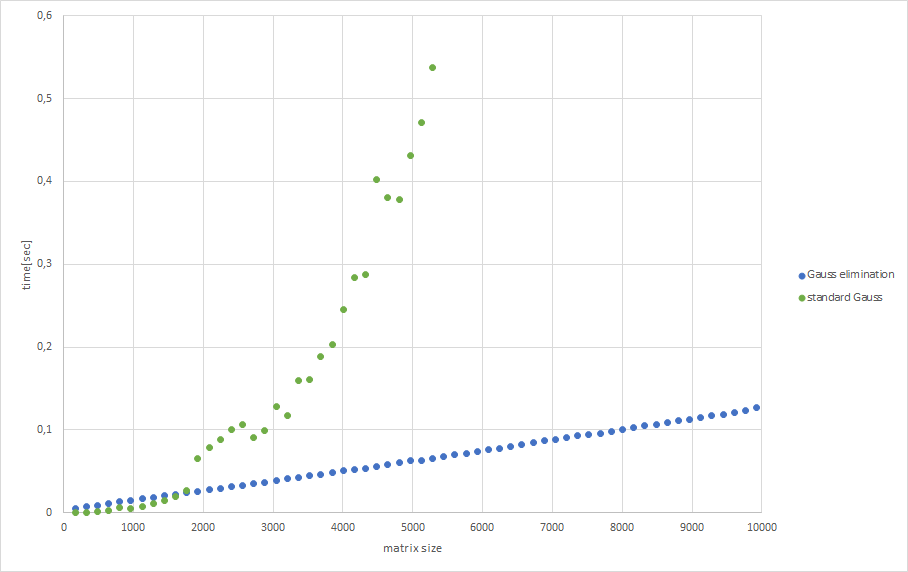
\includegraphics[width=0.5\textwidth]{plots/time4.png}}
		\subfloat[1.][Czas rozwiązywania jednego z układów równań dla tej samej macierzy (100 prób)]{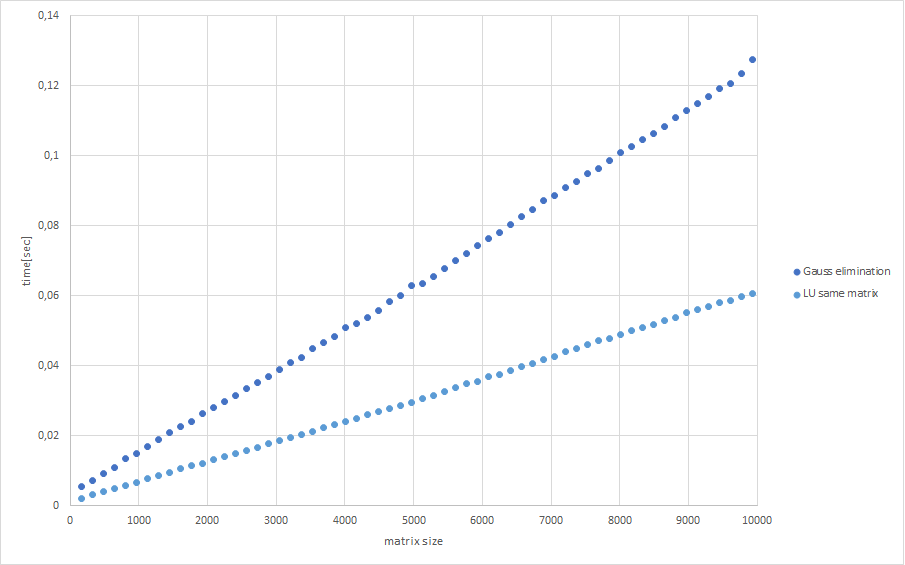
\includegraphics[width=0.5\textwidth]{plots/time3.png}} 
		\caption{}  
		\label{fig:1}  
	
		\subfloat[1.][]{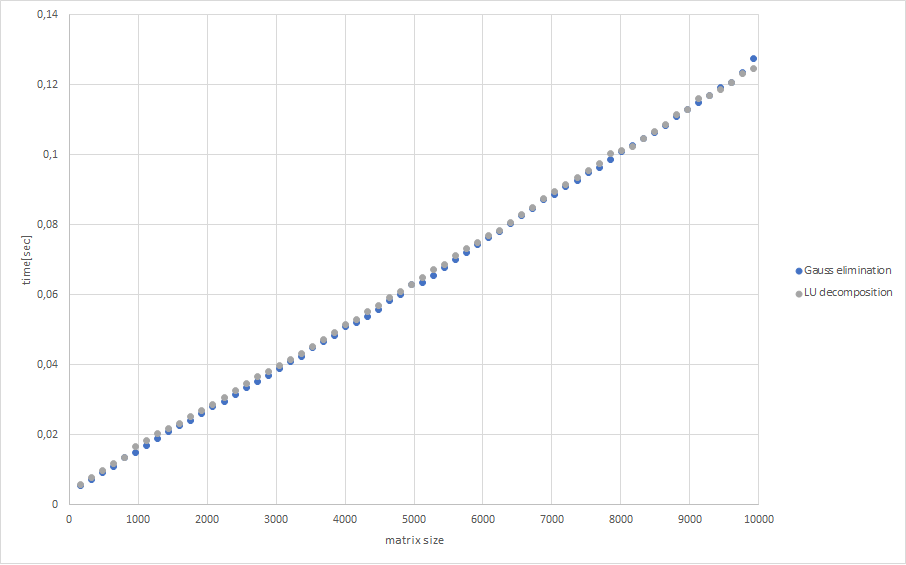
\includegraphics[width=0.5\textwidth]{plots/time1.png}} \hfill
		\subfloat[2.][]{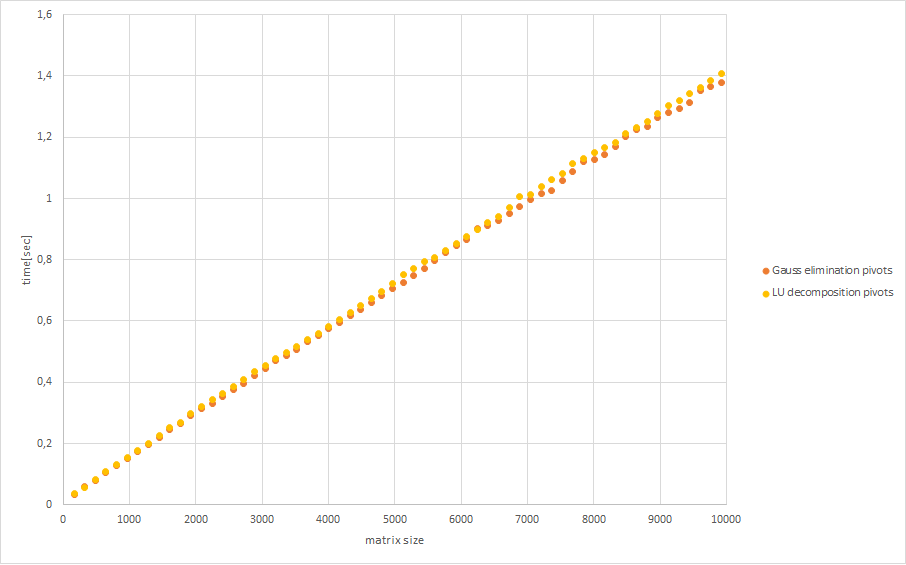
\includegraphics[width=0.5\textwidth]{plots/time2.png}}
		\caption{Złożoność czasowa eliminacji Gaussa i rozkładu LU bez (a) oraz z (b) wyborem elementu głównego.}  
		\label{fig:2} 
		
		\centering
		\subfloat[1.][]{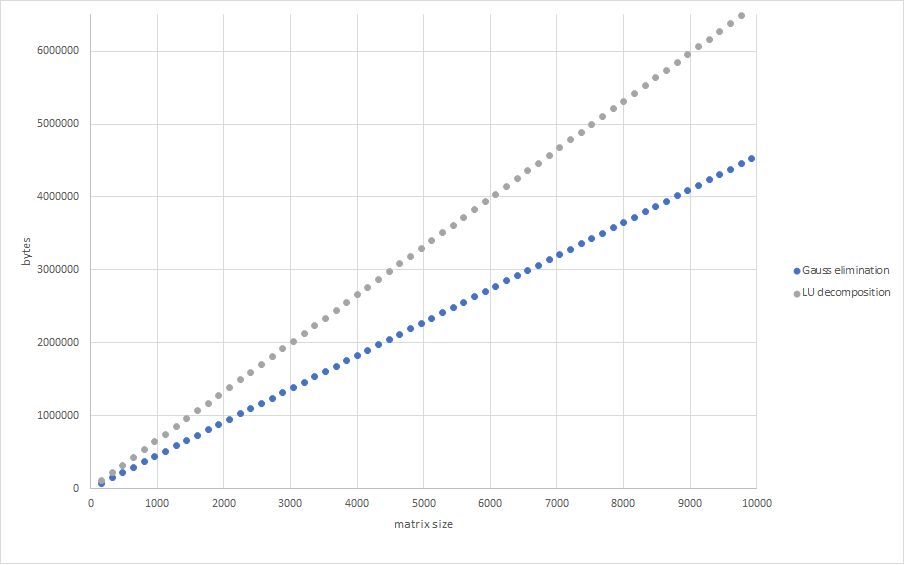
\includegraphics[width=0.5\textwidth]{plots/memory1.png}} \hfill
		\subfloat[2.][]{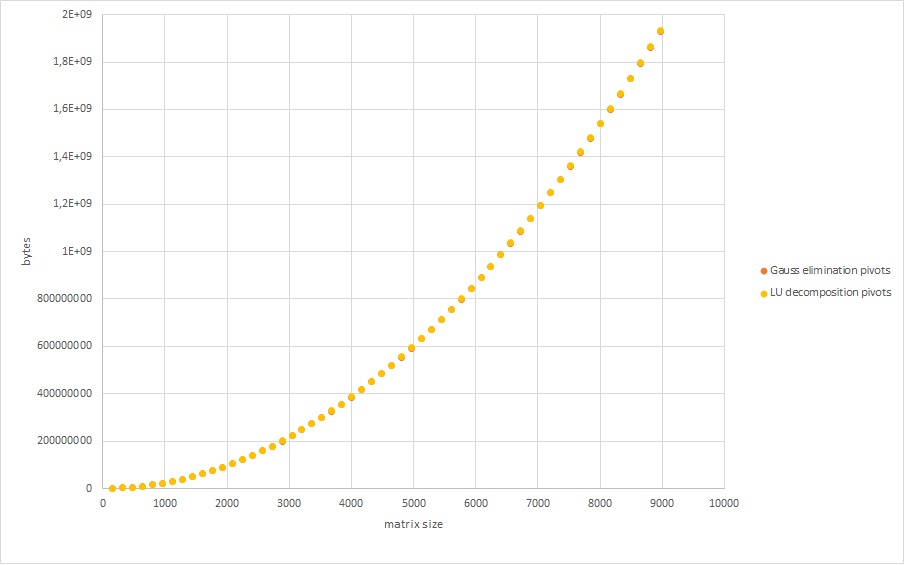
\includegraphics[width=0.5\textwidth]{plots/memory2.png}}
		\caption{Złożoność pamięciowa eliminacji Gaussa i rozkładu LU bez (a) oraz z (b) wyborem elementu głównego.}
		\label{fig:3}
	\end{figure}
	
	\begin{table}[!hpbt]
        		\centering
        		\footnotesize
			\sisetup{
				table-number-alignment = right,
				table-figures-integer = 2,
				table-figures-decimal = 16,
				table-figures-exponent = 2
			}
			\begin{tabular}{|c|S|S|S|} \toprule
				{} & \multicolumn{3}{c|}{Rozmiar macierzy}	\\ \midrule
				{metoda} & {$n=16$} & {$n=10000$} & {$n=50000$} \\ \midrule
				Gauss & 6.383782391594657e-16 & 1.040205776165185e-13 & 1.932760415264822e-13 \\ 
	 			Gauss z wyborem & 3.065703529144609e-16 & 5.320922653862027e-16 & 5.145451947624984e-16 \\
	 			$\mL\mU$ & 8.794620319638098e-16 & 8.968695564214933e-15 & 1.8605011639754745e-13 \\ 
	 			$\mL\mU$ z wyborem & 2.288783399261118e-16  & 5.186001368086655e-16  & 5.031405319253065e-16  \\ \bottomrule
	 		\end{tabular}
	 		\caption{Wartość błędu względnego rozwiązania układu równań z macierzami różnych wielkości dla implementowanych metod.}
			\label{table:1}
		\end{table}
		
\section{Wnioski}
	Poprawność działania zaimplementowanych metod widoczna jest w Tabeli 1 --- uzyskano bardzo niewielkie wartości błędów względnych, przy czym są one zauważalnie mniejsze są dla algorytmów z częściowym wyborem elementu głównego.
	
	Analiza Rysunku \ref{fig:1} (a) pozwala potwierdzić, że przez dostosowanie algorytmu do charakterystycznej postaci macierzy można uzyskać znacznie lepszą złożoność obliczeniową (w tym przypadku udało się uzyskać $O(n)$ z metody o złożoności sześciennej).
	
	Wykresy na Rysunku \ref{fig:2} pokazują, że implementacja rozwiązania zadanego problemu ma wymaganą liniową złożoność obliczeniową. 
	Uzyskane czasy dla metody eliminacji Gaussa pokrywają się z rezultatami przy wykorzystaniu rozkładu $\mL\mU$ oraz analogicznie ma to miejsce dla odpowiadających metod z częściowym wyborem elementu głównego.
	
	Zauważalny jest niemal 12-krotnie dłuższy średni czas rozwiązywania metodami z wyborem elementu głównego niż w przypadku ich standardowych wersji. Jednak pomimo tak drastycznej różnicy warto mieć na uwadze, że wykorzystanie tych wolniejszych wariantów niekiedy może być nieuniknione (np. przy próbie rozwiązania układów z zerami na diagonali).
	
	Złożoność pamięciowa widoczna na Rysunku \ref{fig:3} jest liniowa dla funkcji bez wyboru elementu głównego oraz kwadratowa dla ich wolniejszych wersji --- wynika to najprawdopodobniej z konieczności wypełniania macierzy powodowanego permutacjami wierszy.
	
	Rysunek \ref{fig:1} (b) jasno przedstawia, że wykorzystanie rozkładu $\mL\mU$ jest o wiele efektywniejsze w przypadku rozwiązywania wielu układów równań z tą sama macierzą. Znajduje to swoje teoretyczne potwierdzenie --- etap rozkładu macierzy (eliminacja Gaussa) jest wtedy wykonywany jedynie raz, pozwalając na znaczne obniżenie całkowitego czasu rozwiązywania. 
	
	Problem w trafny sposób pokazuje, że algorytmy rozwiązywania układów równań można zmodyfikować w taki sposób, aby, dostosowane do struktury zadanej macierzy, osiągały o wiele lepszą złożoność obliczeniową.
	
	
\end{document}